% This is samplepaper.tex, a sample chapter demonstrating the
% LLNCS macro package for Springer Computer Science proceedings;
% Version 2.20 of 2017/10/04
%
\documentclass[runningheads]{llncs}
%
\usepackage{graphicx,todonotes, url,soul,graphicx}
\usepackage[square, comma, sort&compress, numbers]{natbib}
\renewcommand\bibname{References}
% Used for displaying a sample figure. If possible, figure files should
% be included in EPS format.
%
% If you use the hyperref package, please uncomment the following line
% to display URLs in blue roman font according to Springer's eBook style:
% \renewcommand\UrlFont{\color{blue}\rmfamily}

\newcommand\rc[1]{\textcolor{red}{#1}}
\newcommand{\upcite}[1]{\textsuperscript{\textsuperscript{\cite{#1}}}}
\begin{document}
%

\title{An Experimental Comparison of Reinforcement Learning Approaches on MOBA\\
} 
%\thanks{Supported by organization x.}}
%
%\titlerunning{Abbreviated paper title}
% If the paper title is too long for the running head, you can set
% an abbreviated paper title here
%
%\author{First Author\inst{1}\orcidID{0000-1111-2222-3333} \and
%Second Author\inst{2,3}\orcidID{1111-2222-3333-4444} \and
%Third Author\inst{3}\orcidID{2222--3333-4444-5555}}
\author{Yu Zhao\inst{1,2}\\
Supervisor: Dr Jialin Liu, Prof. Xin Yao}

%
\authorrunning{Yu Zhao}
% First names are abbreviated in the running head.
% If there are more than two authors, 'et al.' is used.
%
\institute{Department of Computer Science and Engineering\\Southern University of Science and Technology (SUSTech), Shenzhen, China
\and
Lightspeed \& Quantum Studios, Tencent\\
\email{11612908@mail.sustech.edu.cn}
}

%
\maketitle              % typeset the header of the contribution
%
\begin{abstract}
  {MOBA games have developed rapidly in recent years, and many of their features, such as playing strategies, have attracted a large number of players. Correspondingly, due to the large user-population and rich strategies, many studies of Game-AI have also begun to be related to MOBA games. As a player who loves MOBA games, I am very excited to get an internship at Lightspeed \& Quantum Studios (Tencent). I will improve their MOBA environment here so that it can be used to train MOBA AI and study some algorithms for reinforcement learning.}

\keywords{MOBA \and Reinforcement learning \and Game AI \and Multi-scenario.}
\end{abstract}
%
%
%
\section{Introduction}
\subsection{Introduction of MOBA game}
\qquad MOBA (multiplayer online battle arena) refers to multiplayer online technical competitive games, such as League of Legends and Glory of Kings. In the game, ordinary players are divided into two groups to compete, and each player controls a hero to play the game with the goal of destroying the opponent's base.
\subsection{AI training on famous MOBA games}
\qquad For current research, "OpenAI has used the multiplayer video game Dota 2 as a research platform for general-purpose AI systems. At April 13, 2019, OpenAI Five won back-to-back games versus Dota 2 world champions OG at Finals, becoming the first AI to beat the world champions in an esports game."\upcite{OpenAI-Blog}

From OpenAI's Blog\upcite{OpenAI-baselines-ppo}, the main algorithm for reinforcement learning is Proximal Policy Optimization Algorithms.\upcite{OpenAI-PPO} DeepMind also published their article Emergence of locomotion behaviours in rich environments\upcite{Deep-Mind}. Both of them are based on Trust region policy optimization\upcite{2015} which is published in 2015. It shows that distributed PPO has become the most popular algorithm in reinforcement learning.
\subsection{Importance of a suitable platform for training}
\qquad For training MOBA AI, a suitable training platform is very important. If we directly choose to use a large game such as DOTA2 as a training platform, since we need to use all the functions, we may need too many parameters for training, so the amount of calculation we train will be huge. And if we do training in a simple MOBA environment, we can abandon many unnecessary elements, such as team fights in simple scenes, we should not add towers and fog of war so that the amount of training is reduced and it is more convenient for us to observe the results and modify the algorithm (if the training time is too long, it will take too long to verify an algorithm modification).

\subsection{Motivation}
\qquad As a TOP500 Dota2 player, I was shocked to see that OG lost to OpenAI Five. When OpenAI allowed everyone to team up to compete with it, some of my national service TOP200 friends and I tried to challenge it but failed. This got me interested in training my AI on the MOBA platform and verifying some of the algorithms used by OpenAI Five.
\subsection{Tasks}
\begin{enumerate}
\item Improvement of the MOBA game environment: Compared with mature MOBA games (such as League of Legends), improve the hero skills and scene logic in the MOBA game, such as the fog of war and the towers.\\

\item Research on AI in MOBA games: Perform some reinforcement learning algorithm verification in the MOBA environment in Task 1, such as distributed PPO, and verify the effects of some deep network structures, such as LSTM and self-encoding
\end{enumerate}
\subsection{Contribution}
\subsubsection{Current work}
The current stage mainly completed the improvement of the MOBA environment  and added some training scenarios such as kite flying for subsequent training.\\
\begin{enumerate}
\item At present, towers can be used in MOBA-env. Towers are very important for decision-making in MOBA games. There are many-to-many agent training around towers in future training scenarios.\\
\item The kiting scene is relatively common and simple. The carry hero who moves fast and has a long attack distance completes the killing of the bulky hero by "hit and run". The purpose is to learn to build the scene and familiarize with the training session and observe the training output through this scene.
\end{enumerate}
\subsubsection{Future work}
\begin{enumerate}
\item {\hl {Construct more scenes for training.\\}}
\item{\hl {Use the constructed scene to complete the verification of the distributed learning algorithm (distributed PPO). Through the training in the same scene, observe the changes of training efficiency and training effect.}}
\end{enumerate}

%\todo[inline]{Outline gives here (one paragraph)}
%The remainder of this paper is organised as follows. Section ...


\section{Background}

\subsection{Multiplayer Online Battle Arena (MOBA)}
\qquad MOBA (multiplayer online battle arena) refers to multiplayer online technical competitive games, such as Dota2, League of Legends, King of Glory, etc.

The MOBA game is not only popular because of its fairness and thresholdlessness, but also because of its real-time strategy and long-term strategy. Most of the young enjoy playing one or more MOBA games, for example, King of Glory has 100 million monthly online.

\subsection{Existing Platform/Benchmark for MOBA}
\qquad The more famous MOBA environment currently available for training AI is DOTA2, because it provides some interfaces to control the actions of heroes. Its advantages are very obvious: first, the interface is ready, you don't need to read the game source code or even write the game source code yourself; second, the game logic is ready, you don't need to write the logic of the towers and the fog of war and the calculation of damage formula. The disadvantages of using DOTA2 as a platform: the calculation number of each step during training is too large, too many parameters, the time required for training once is too long, it is not convenient to observe the results, and the workload of debugging is huge.\\

Outside of DOTA2, openAI's gym \upcite{1606.01540} is also providing a good platform for training MOBA AI. Although the gym given by OpenAI needs to define its own character model, and the skills and game logic also need to be designed by users, the advantages of OpenAI's gym are also obvious. First, it only needs to implement a part of the game logic that user need, which greatly reduces the amount of calculating so that the speed of training will become faster. Second, it allows users to modify gym data, users can define heroes and skills themselves.

\subsection{Reinforcement Learning for MOBA}
\qquad From OpemAI's blog\upcite{OpenAI-baselines-ppo}, PPO has become OpenAI's alternative algorithm for reinforcement learning. If one sentence summarizes PPO: OpenAI proposes a solution to the problem that the policy gradient does not determine the learning rate (or step size). If the step size is too large, the learned policy will always be chaotic and will not converge, but if the step size is too small, we will wait for despair to complete the training. PPO uses the ratio of the new strategy to the old strategy, which limits the update range of the new strategy and makes Policy Gradient less sensitive to slightly larger step sizes. But OpenAI haven't publish the algorithms they use when training OpenAI Five, so I want to use the distributed PPO algorithm to test the effect of MOBA-AI in the MOBA-env environment\upcite{OpenAI-PPO}.\\

The part we can optimize on the algorithm is that some deep networks such as LSTM\upcite{LSTM} can be added, because MOBA games have not only short-term decisions but also long-term decisions. If we add LSTM, we infer that Agent's long-term decision-making will become better.\\

Deep-Mind also implemented their Distributed PPO algorithm as we have mentioned in the introduction. If time permits, I would also like to observe the differences in the efficiency and effectiveness of DPPO training between Open-AI and DeepMind.\upcite{Deep-Mind}

\section{Platform: MOBA-env(based on OpenAI gym)}
\qquad MOBA-env\upcite{MOBA-env} is a mini MOBA game, which can be integrated into gym env. Users can use this env to train AI for MOBA game.
\subsubsection{Structure of MOBA-env}
MOBA-env's game logic is written in Go. In a directory, users can easily use the go build ./ command to compile. Users can also make changes to the game logic according to their needs. gym-MOBA is the folder containing the interface needed to integrate the gamecore logic into gym env. These two parts contains what we can do for the game(add heroes, change game logic, change interfaces).
The current training code is written in Python3 using tensorflow\upcite{tensorflow} framework.

\subsubsection{Limitation of the current platform}
The current limitations of MOBA-env are too few heroes, too few scenes, and imperfect game logic. Too few heroes will reduce the number of scenarios that users can train, and it is inconvenient to observe the training results in multiple scenarios. The imperfect game logic means that unlike the mature MOBA games, it lacks game logic such as the fog of war, which is one of the reasons for too few training scenarios.

\section{Experimental progress}

\subsection{Add new heroes}
\qquad I have added some heroes to MOBA-env for later scene construction. 
\subsubsection{Experimental setting} This game is written in Go language, and the hero information is stored in json format. I first designed the heroes' base data according to the needs of the first scene. Make sure our heroes can't beat the opposite heroes without training, and it is possible to win the opposite heroes when our heroes are controlled by human.
\subsubsection{Experimental results} The result that only the hero has no scene is difficult to show, because in the simple MOBA environment of MOBA-env we did not model the appearance of the hero. So the results of building a new hero will be shown with the new scene in Task {Create a new scene}

\subsubsection{Discussion}
The heroes have been successfully added to MOBA-env, the specific effects and conclusions will be displayed and discussed in Task {create a new scene}.
\subsection{Created a new scene}
\qquad I have created a simple scenario to train a kite-flying strategy using the new hero constructed above.

\subsubsection{Experimental setting} This scene is used in conjunction with the above heroes. In addition to considering the hero's panel value when designing, I also need to consider the size of the map, whether to use towers, creepers or other factors. Since the aim is familiar with the environment construction scene, I did not set up defense towers and soldiers, only the heroes move or attack on the map according to the decision.


\subsubsection{Experimental results}

When the gym inits, heroes are randomly distributed on the map (because it is a simple scene, I did not configure a defense tower and soldiers):\\
\begin{figure}
	\centering
	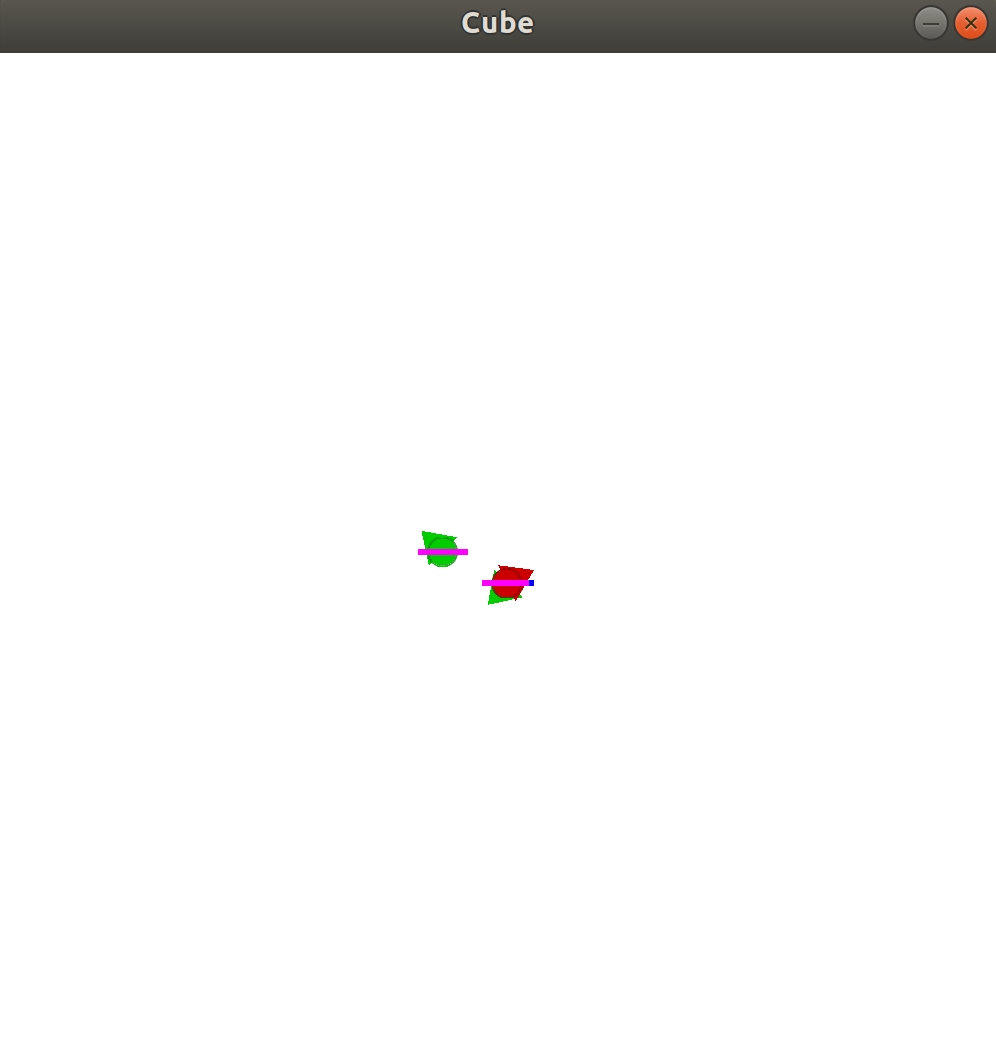
\includegraphics[width=0.50\textwidth]{1.jpg}
	\caption{Initial state, the whole window is the map, the green and the red are different camps. Each hero has the current direction of movement and health, purple for retained health, and blue for reduced health.}
\end{figure}
\\
Briefly introduce through Fig.1, green and red represent different camps, the purple of the blood bar represents the remaining health (the upper left corner is full health), and the blue represents the health that has been deducted. In this picture, the green and purple encounter each other. The attack resulted in a health reduction, with a blue portion of the blood strip.

Firstly, as the health and attack power's gap is too large, the green camp looks helpless, see Fig.2, Fig.2 shows that without a reasonable strategy the green camp will lose.
\begin{figure}
	\centering
	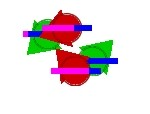
\includegraphics[width=0.50\textwidth]{2.jpg}
	\caption{Without suitable strategies, the green heroes don't have health, red will win.}
\end{figure}


When I control the green(Use keyboard input to call the interfaces in gym-MOBA), green camp can win finally, see Fig.3, Fig.4:

\begin{figure}
	\centering
	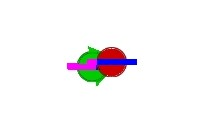
\includegraphics[width=0.50\textwidth]{3.jpg}
	\caption{Red is no health because of reasonable strategies. }
\end{figure}

\begin{figure}
	\centering
	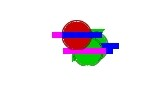
\includegraphics[width=0.70\textwidth]{4.jpg}
	\caption{Red is no health because of reasonable strategies.(2)}
\end{figure}

This shows that with a reasonable strategy the green camp will win. \\ \\ \\

\subsubsection{Discussion}
From Fig.1-4 we can see that the hero I defined can complete normal movement instructions and attack instructions in MOBA-env. And the kiting scene I designed is reasonable because when the kite flying strategy is not adopted, there is no doubt that the green will lose due to the difference between the upper limit of health and the attack power; but if the kite flying strategy is used, due to the moving speed and attack distance The advantage of green is clearly that it can win, and red has no winning strategy.


\section{Conclusion}
\qquad So far, I have added new heroes and new scenes to MOBA-env and became familiar with the training process. The data of these heroes is completely designed by myself, and the scenes are completely configured by myself. After configuring the scene, I used the play-game mode (AI does not control the agent) and found that the kite flying scene I configured is feasible, that is, we will lose without a right strategy, but under a reasonable strategy we can win. The advantages of the scene I made is that the amount of calculation required for training is relatively small, you can quickly see the training results, and you can understand some details of the training code through this simple scene. The configuration of this scene can still be used in other scenarios. For example, in a 5v5 team fight, the carry hero may need to use a kite-flying strategy to dodge the opponent while attacking, and the front row meat shield hero may need to use a more reasonable strategy to achieve team protection.\\ \\ \\

\section{Future Work}
\begin{enumerate}
\item Continue to build more scenes. With the previous pavement and familiarity with the environment, this step will be simple. I will try to build more scenes. The current scenes cannot build a hero-to-hero training scene. I will read the protocol of Open-AI gym and try to solve it.\\
\item Read related papers about distributed PPO and LSTM and learn about distributed PPO and LSTM. Most of them have been mentioned at the background.\\
\item Verify the distribute PPO algorithm. Observe reward, step size, convergence speed and other values.\\
\item Verify the effect of deep network structures (e.g. LSTM).Observe reward, step size, convergence speed and other values.
\end{enumerate}
%
% ---- Bibliography ----
%
% BibTeX users should specify bibliography style 'splncs04'.
% References will then be sorted and formatted in the correct style.
%
% \bibliography{main}
\bibliographystyle{ieeetran}
\bibliography{main}
%
\end{document}
